\begin{frame}
    \begin{center}
        
\includegraphics[width=\textwidth]{figures/wrestlingPFAS.png}
    \end{center}

    \Huge\bf
    \textcolor{msred}{
    PFAS - the Immortal}
\end{frame}

\begin{frame}{What's a PFAS?}
    \Huge\centering
    \textcolor{msred}{\bf P}er- and
    poly\textcolor{msred}{\bf F}luoro\textcolor{msred}{\bf A}lkyl
    \textcolor{msred}{\bf S}ubstances
\end{frame}

\begin{frame}
    \center \includegraphics[width = .8\textwidth]{figures/RPU
    Products Containing PFAS.jpeg}
    \captionof*{figure}{\footnotesize Infographic by the Californian government}
\end{frame}

\begin{frame}
    \begin{minipage}{\textwidth}
        \center 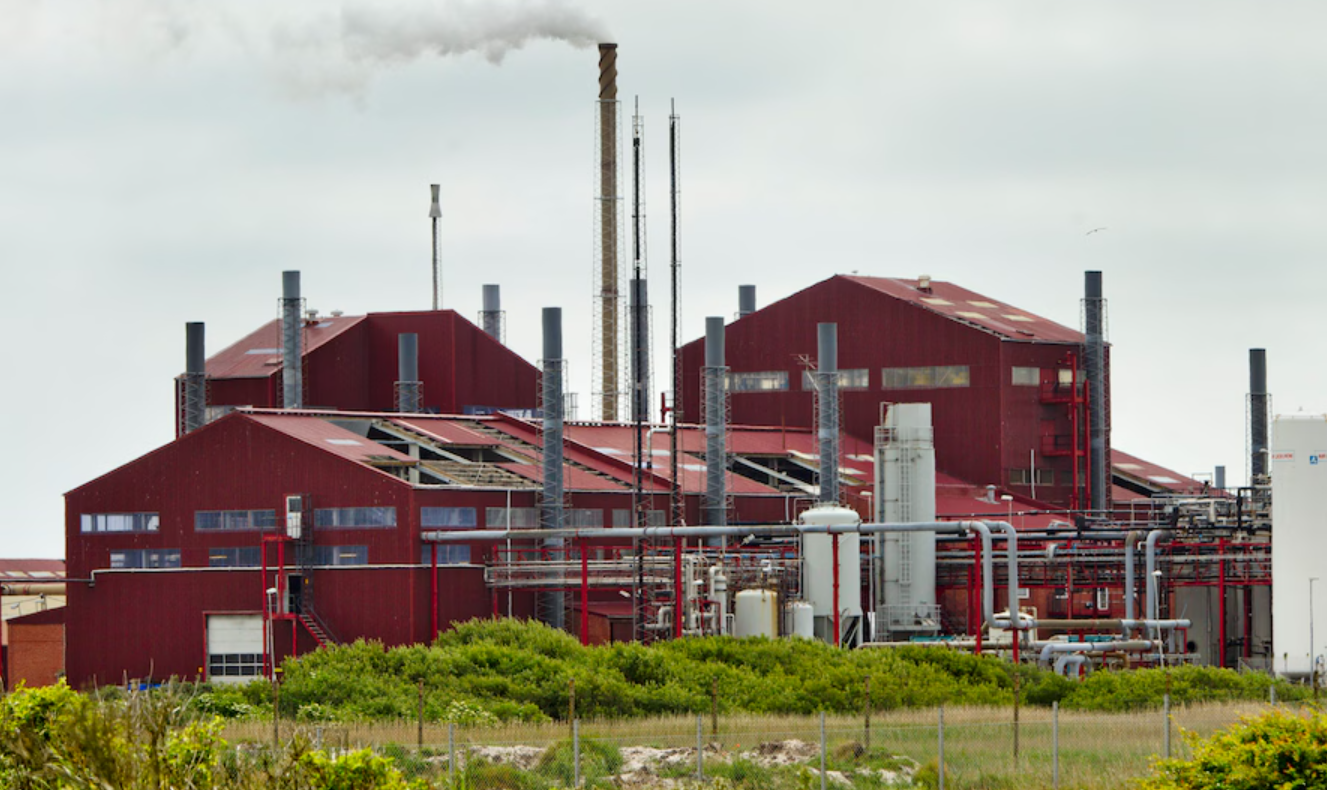
\includegraphics[width = .8\textwidth]{figures/cheminova.png}
    \end{minipage}

    \begin{minipage}{\textwidth}
        \center 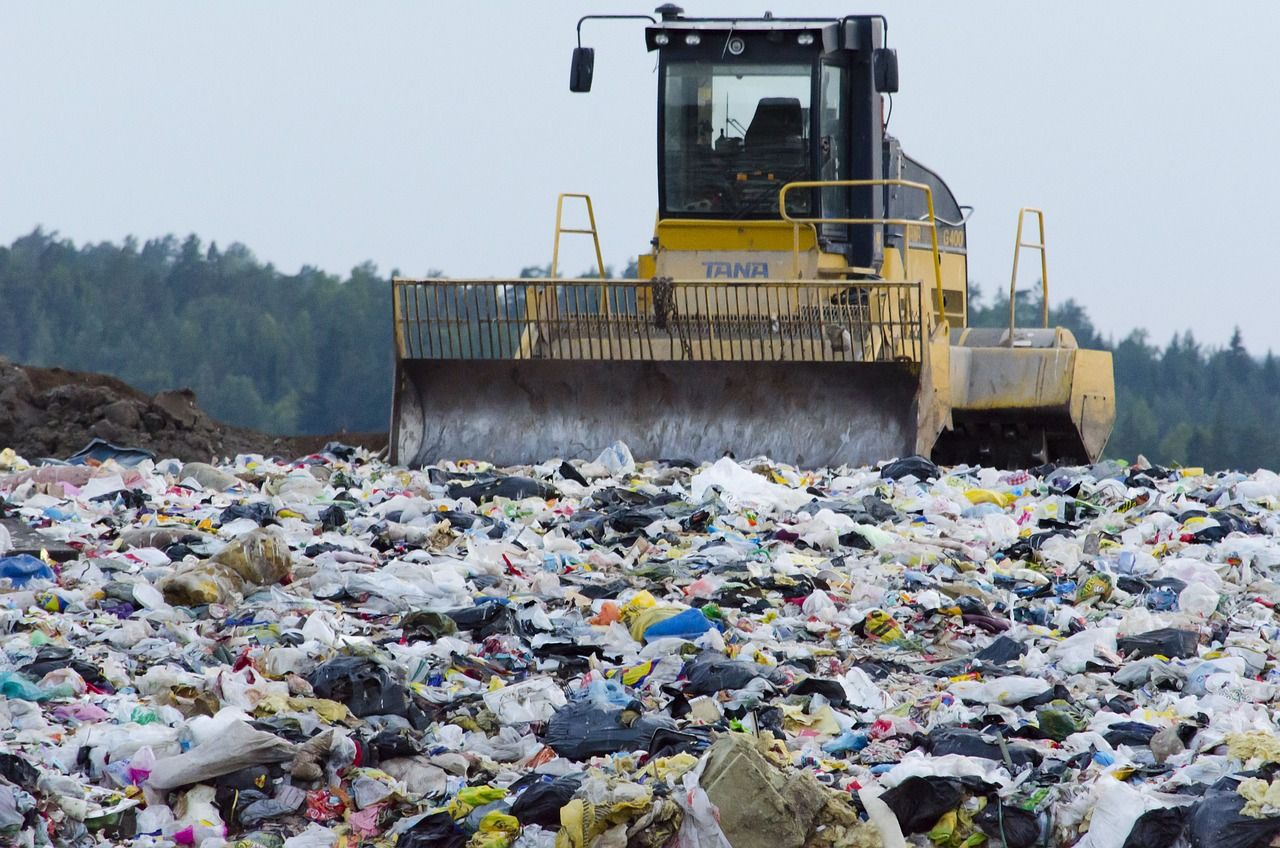
\includegraphics[width = .8\textwidth]{figures/landfill.jpg}
    \end{minipage}
\end{frame}

\begin{frame}{Where do they live?}
    \textbf{Where DON'T they live!?}
    PFAS are found in water, air, fish, and soil..\pause

    Also, in blood of people, animals, in food
    products\footnote{\url{https://www.epa.gov/pfas/pfas-explained}}

\end{frame}

\begin{frame}{What they do to
    us\footnote[frame]{\tiny\url{https://www.epa.gov/pfas/our-current-understanding-human-health-and-environmental-risks-pfas}}}

    \begin{itemize}
        \item Decreased fertility, effects on pregnant people
        \item Developmental effects or delays in children,
        \item Risk of some cancers, prostate, kidney, testicular.
        \item Impact on immune system, infections, reduced vaccine response.
        \item Interference hormones.
        \item Increased cholesterol - risk of obesity.
    \end{itemize}
\end{frame}

\begin{frame}{PFAS measurements in groundwater wells}
    \centering
    \center 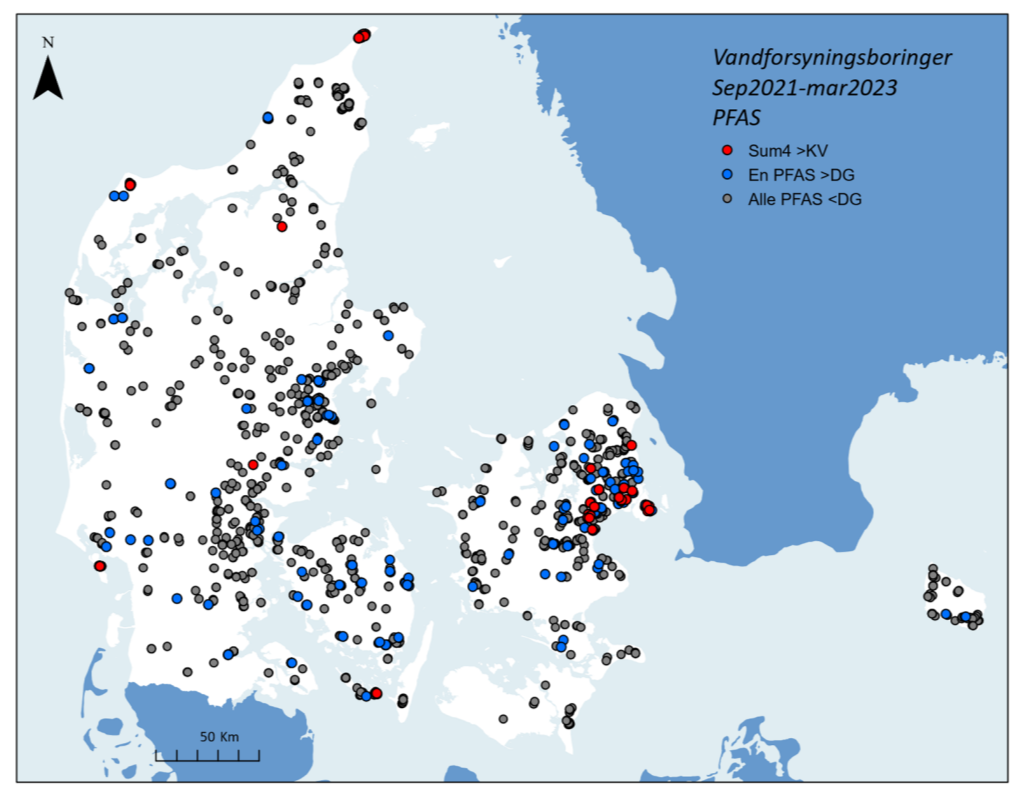
\includegraphics[width = .75\textwidth]{figures/pfasMeas.png}

    \captionof*{figure}{\footnotesize\emph{Red:} PFAS chemicals above limit.
        \emph{Blue:} Measured PFAS chemicals. \emph{Grey:} None
    detected~\cite{anders_r_johnsen_laerke_thorling__christian_n_albers_pfas-stoffer_2023}.}

\end{frame}

\begin{frame}{PFAS measurements in groundwater wells}
    \centering
    \center 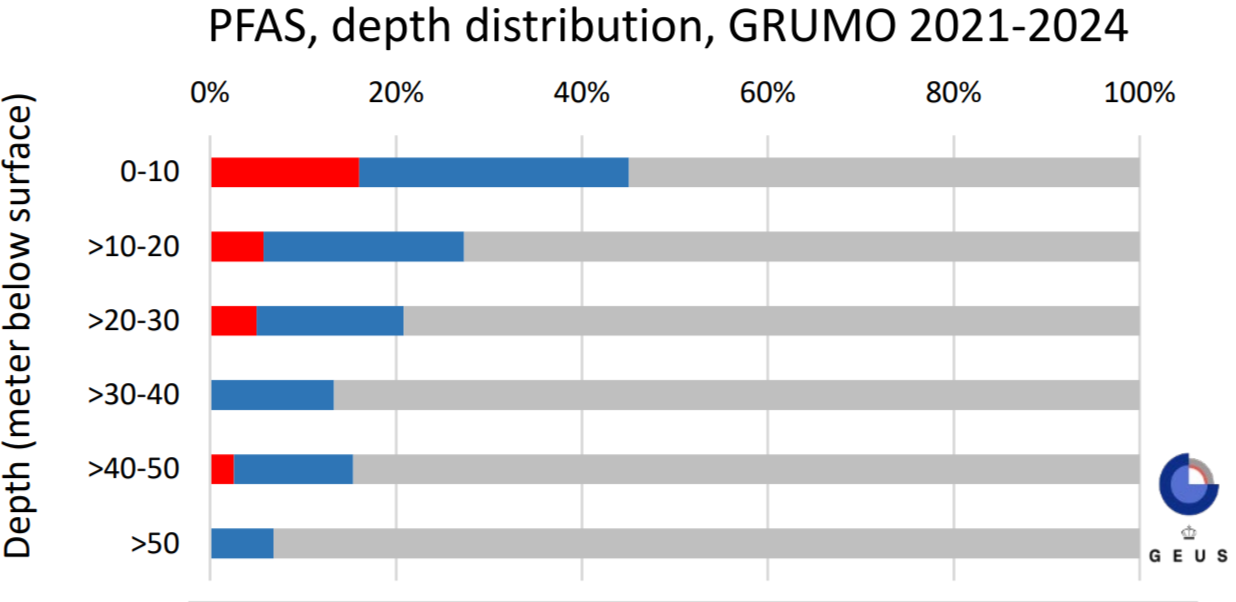
\includegraphics[width = .75\textwidth]{figures/pfasdepth.png}

    \captionof*{figure}{\footnotesize\emph{Red:} PFAS chemicals above limit.
        \emph{Blue:} Measured PFAS chemicals. \emph{Grey:} None
    detected~\cite{laerke_thorling_groundwater_2025}.}

    PFAS does not simply break down. They're the eternity chemicals.
\end{frame}
